\newpage
\section{NOTA TEÓRICA}

Antes de iniciar con el uso y manipulación del lenguaje de programación C para la creación de los algoritmos objetivo del presente laboratorio, es necesario tener a mano una serie de conceptos importantes, los cuales se explican a continuación: 

\subsection{Arduino UNO}
\subsection{Microcontrolador ATM328P}%Micro de la placa Arduino UNO
Tal como se detalla en la hoja del fabricante \cite{AT}, este componente corresponde a un microcontrolador de 8 bits, de alto rendimiento y de baja potencia, producido por la empresa Atmel. Cuenta con 131 instrucciones, una memoria flash con capacidad de 32 kb, una SRAM de 2Kb y una memoria EEPROM de 1 Kb. Asimismo, cuenta con 23 GPIO programables, 3 timers (dos de 8 y otro de 16 bits), seis canales PWM, además de SPI y una USART \textit{full duplex}. En la Figura \ref{fig:AT_pins} puede observarse la distribución de pines del microcontrolador y sus respectivas funciones:  

\begin{figure}[H]
\centering
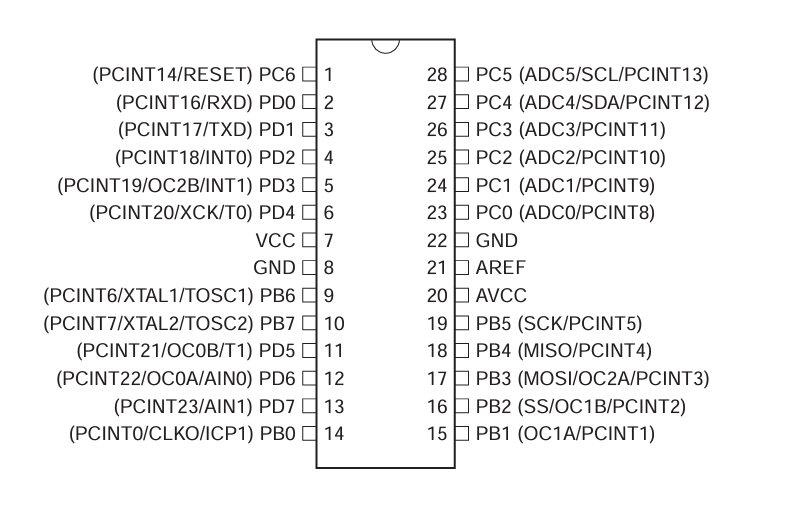
\includegraphics[width=140mm]{./Figuras/Nota_teorica/PINES}
\caption{Diagrama de pines y sus respectivas funciones. (Fuente: Imagen tomada de \cite{AT})}
\label{fig:AT_pins}
\end{figure}

 Para más información general del dispositivo, observar el Anexo \ref{an:01_GEN}. 
Por otro lado, en la Figura \ref{fig:DBLO} puede consultarse el diagrama de bloques del microcontrolador en el cual puede consultarse a alto nivel la conexión interna de este (no incluye el CPU):

\begin{figure}[H]
\centering
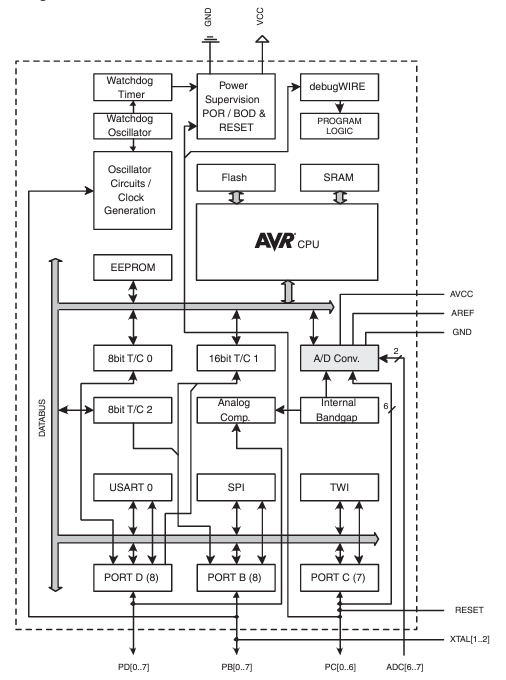
\includegraphics[width=160mm]{./Figuras/Nota_teorica/Bloques}
\caption{Diagrama de bloques del ATtiny4313. (Fuente: Imagen tomada de \cite{AT})}
\label{fig:DBLO}
\end{figure}



\subsubsection{Registros de importancia}
  A diferencia de otros microcontroladores, Arduino busca hacer la programación y el desarrollo de proyectos de hardware más accesible para una amplia gama de personas. Por lo tanto, se enfoca en proporcionar una capa de abstracción más alta sobre el hardware, lo que significa que no es necesario manipular los registros del microcontrolador directamente en la mayoría de los casos.

\subsection{Librerías de importancia}

\subsubsection{PCD8544}
PCD8544 es una biblioteca de software diseñada para Arduino, que permite controlar fácilmente la pantalla Nokia 5110 que cuenta con una resolución de 48x84 píxeles. Esta pantalla es comúnmente utilizada por su bajo costo y bajo consumo, lo que la hace óptima para proyectos y prototipos. La librería proporciona a los desarrolladores una serie de funciones para interactuar con la pantalla, inicializar la pantalla, ajuste de contraste y temperatura, dibujar pixeles, lineas, cuadros, texto de distintos tamaños son algunas de las funcionalidades. Dado que esta destinada para Arduino, su uso es muy intuitivo, esto permite al usuario centrarse en la logica de su aplicación \cite{Rodrigues}.

\subsubsection{PID\_v1\_bc}
Esta librería es una versión mejorada de la librería PID, pues se añade una tecnica llamada  back calculation que se refiere a un método específico para manejar el windup del integrador en controladores PID. Esta librería ofrece una forma sencilla de integrar este tipo de control PID en proyectos de Arduino, proporcionando una interfaz para configurar los parámetros del controlador PID \cite{Forrest}.

\subsection{Resistencia de \textit{pull-down}}\label{sec:cir0}
Del enunciado del laboratorio, se sabe que el objetivo de este es construir un simulador de un paso peatonal que cuente con dos botones de entrada con los que el usuario pueda solicitar una parada del tránsito vehicular. De lo anterior se puede deducir que al menos uno de los pines del microcontrolador debe ser configurado como entrada y que esta debe permanecer en un estado determinado, para que sólo en caso de presionar el botón (se obtiene el inverso del estado anterior), se active su funcionamiento. Para ese diseño, se quiere que el estado por defecto sea en bajo para proteger el circuito constantemente y que el estado en alto (al presionar el botón) active el circuito. 

Una resistencia de pull-down permite lograr el comportamiento deseado para el caso expuesto. En la Figura \ref{fig:pullD} puede observarse la disposición adecuada construida en SimulIDE según se detalla en \cite{pullU}: 

\begin{figure}[H]
\centering
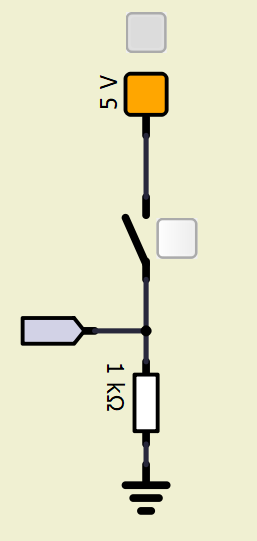
\includegraphics[width=40mm]{./Figuras/Nota_teorica/pullD}
\caption{Ejemplo de resistencia de \textit{pull-down} y \textit{switch} en SimulIDE.}
\label{fig:pullD}
\end{figure}

En la Figura \ref{fig:pullD}, puede observarse como el pulsador está conectado entre la fuente de tensión y el pin del MCU. Cuando el interruptor es presionado, la entrada del microcontrolador está en un valor lógico alto, pero cuando el interruptor está abierto, la resistencia \textit{pull-down} ``jala'' la tensión de entrada a la tierra (valor lógico cero). Según se explica en \cite{pullU}, la resistencia \textit{pull-down} debe ser mayor que la impedancia de salida del dispositivo, ya que de lo contrario podría ser capaz de bajar la tensión demasiado y la tensión de entrada en el pin se mantendría en un valor bajo lógico constante. Para calcular esta, se aplica la ley de Ohm de la siguiente forma: 

\begin{equation}
    Z_{MCU} = \frac{V_{DD}}{I_{max}}
\end{equation}

Donde $V_{DD}$ corresponde a la tensión máxima entregada por cada pin del MCU y $I_{max}$ la corriente máxima en el mismo caso, de esta forma se tiene que: 

\begin{equation}
    Z_{MCU} = \frac{5}{20 \times 10^{-3}} = 250 \; \Omega
\end{equation}

Para este caso particular, se tomará su valor como 1 k$\Omega$ para asegurarse de que no haya ningún problema.

\subsection{Circuito para lidiar con el \textit{switch bounce}} \label{sec:cir1}
Tal como se detalla en \cite{RC}, cerrar un \textit{switch}, puede parecer que este hace contacto de manera absoluta e inmediata, sin embargo, este dispositivo no deja de ser mecánico y el contacto ocurre de manera oscilante, por lo que una serie de interferencias son ingresadas a la señal transmitida. Para solucionar este problema, puede utilizarse un circuito RC a la salida del interruptor, de tal forma que se filtren los picos producidos por las oscilaciones y suavicen la señal que será transmitida. Lo anterior es útil para evitar falsas pulsaciones. Un ejemplo del tipo de circuito a construir es el que puede observarse en la Figura \ref{fig:RC1}: 

\begin{figure}[H]
\centering
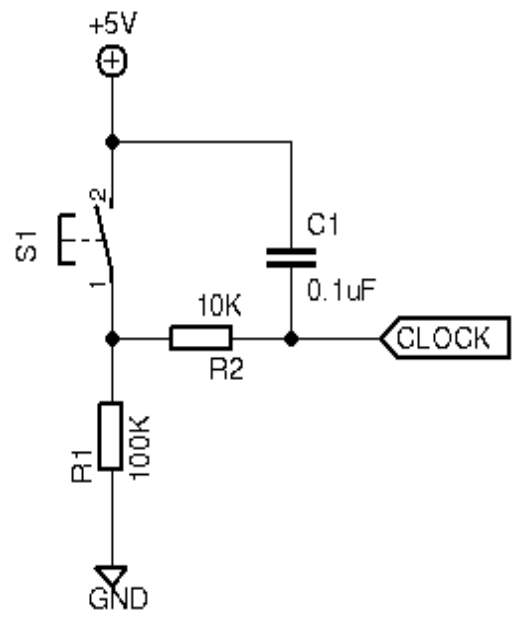
\includegraphics[width=80mm]{./Figuras/Nota_teorica/RC1}
\caption{Ejemplo de circuito utilizado para evitar las oscilaciones producidas por un \textit{switch} que combina un circuito RC con un resistor de \textit{pull-down}. (Fuente: Imagen tomada de \cite{RC})}
\label{fig:RC1}
\end{figure}

Para hacer los cálculos adecuados de capacitancia y resistencia, se inicia definiendo un tiempo de carga y descarga adecuado. En este caso, como no se trata de una acción que necesite de actividad inmediata, se puede trabajar en el orden de los milisegundos, en este caso, de los 100 ms. Como bien se sabe: 

\begin{equation}
    \tau = R \cdot C
\end{equation}

Por lo que si ya se tiene un valor de tiempo, basta con seleccionar una de las dos variables restantes para despejar la otra. Si se toma un valor de resistencia de 5 k$\Omega$, entonces despejando:

\begin{equation}
    C = \frac{\tau}{R} = \frac{10 \times 10^{-3}}{5 \times 10^{3}} = 2 \; \mu F
\end{equation}

\noindent Para apegarse a los valores disponibles en el mercado, se elige un capacitor de 2.2 $\mu$F. 

El circuito resultante construido en SimulIDE puede consultarse en la Figura \ref{fig:RC2} a continuación: 

\begin{figure}[H]
\centering
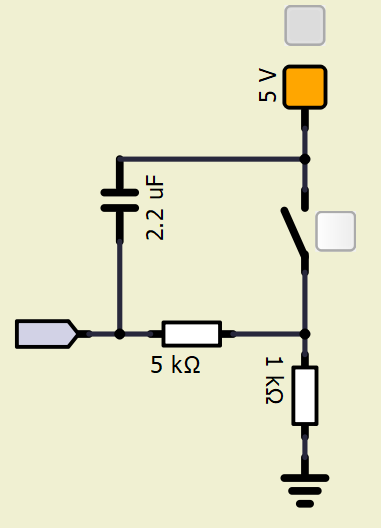
\includegraphics[width=70mm]{./Figuras/Nota_teorica/RC2}
\caption{Circuito utilizado para evitar las oscilaciones producidas por un \textit{switch} que combina un circuito RC con un resistor de \textit{pull-down}.}
\label{fig:RC2}
\end{figure}



\subsection{Diseño del circuito simulador de una incubadora} \label{sec:cir2}
Según se indica en el enunciado, el presente laboratorio tiene como objetivo simular el funcionamiento de un una incubadora de huevos automática basada en el Arduino UNO. 
\begin{figure}[H]
\centering
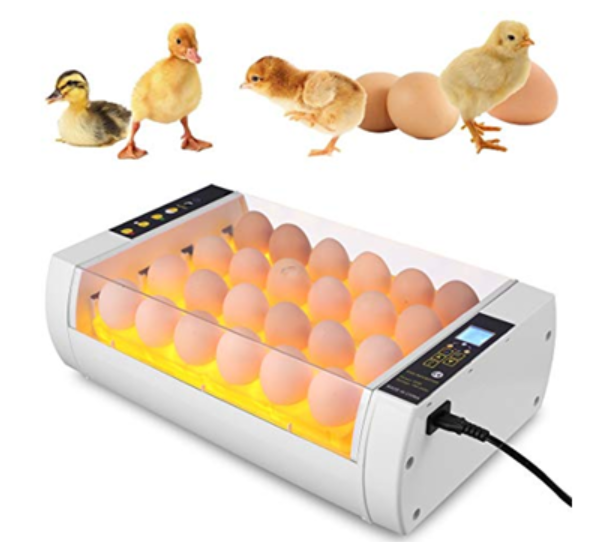
\includegraphics[width=95mm]{./Figuras/Nota_teorica/enun}
\caption{Incubadora Automática.}
\label{fig:enun}
\end{figure}

Algunas de las características solicitadas en el diseño importantes para la construcción del circuito son poder visualizar la temperatura en una pantalla LCD PCD8544, utilizar un potenciómetro para establecer la temperatura de operación, encender un LED de alarma color azul si la temperatura de la incubadora (T) es menor a 30°C, encender un LED de alarma color rojo si T $>$ 42°C, encender un LED color verde si 30°C $\leq T \leq$ 42°C, un \textit{switch} para habilitar la comunicación con la PC y otro para habilitar la impresión en la pantalla LCD.



De la características solicitadas se sabe que habrán 3 LEDs conectados entre alguno de los pines del Arduino y la tierra, por lo que estos necesitan de resistencias de protección. Para calcular el valor de estas, se debe tomar en cuenta que la tensión máxima de operación es de 5 V y la corriente máxima suministrada es de 20 mA, información tomada de la hoja del fabricante \cite{AT}. Para obtener el valor de la resistencia de protección utilizando la ley de Kirchhoff de esta forma:

\begin{equation}
    R = \frac{V_{DD} - V_{LED}}{I_{max}} 
\end{equation}

Como se trata de una simulación, se tomará $V_{LED}$ = 2.4 V (tensión de umbral del simulador) para todos los casos. Para no presionar el sistema, se realizarán los cálculos utilizando 18 mA. De esta forma: 

\begin{equation}
    R = \frac{5 - 2.4}{18 \times 10^{-3}} = 144.44 \; \Omega
\end{equation}

\noindent Es este caso, se selecciona un valor estándar de 150 $\Omega$. 
Para lo que sería la conexión de la pantalla LCD Nokia 5110 a arduino, simplemente se debe conectar según se establece en la documentación de la librería PCD8544.\cite{Rodrigues} A continuación una tabla con los respectivos pines de Arduino y la pantalla:

\begin{table}[H]
\caption{Conexión de pines pantalla-arduino}
\begin{center}
\begin{tabular}{c|c}
\hline
\textbf{Pines LCD NOKIA 5110}&\textbf{Pines Arduino UNO}\\
\hline
RST  & 7\\
CE & 6 \\
DC & 5 \\
Din & 4\\
CLK  & 3 \\
\hline
\end{tabular} \label{table:pantalla}
\end{center}
\end{table}

\subsection{Lista de componentes y precios}

En la Tabla \ref{table:Equipo} pueden consultarse los componentes utilizados y sus precios, tomando como referencia los precios del sitio web de la tienda de componentes MicroJPM (\url{https://www.microjpm.com/}): 

\begin{table}[H]
\caption{Lista de componentes.}
\begin{center}
\begin{tabular}{c|c|c}
\hline
\textbf{Componente}&\textbf{Cantidad}&\textbf{Precio}\\
\hline
Placa Arduino UNO & 1 & \$19,90\\
Switches & 2 & \$0,30\\
Capacitor de 2.2 $\mu$F & 2 & \$0,35\\
Resistor de 5 k$\Omega$ & 2 & \$0,07\\
Resistor de 1 k$\Omega$ & 2 & \$0,07\\
Resistores de 150 $\Omega$ & 3 & \$0,13\\
LED azúl & 1 & \$0.14\\ 
LED verde & 1 & \$0.51\\ 
LED rojo & 1 & \$0,51\\ 
Pantalla LCD & 1 & \$7,50\\ 
Potenciómetro 1K & 1 & \$1,00\\ 
\hline
Total & - & \$31.53\\
\end{tabular} \label{table:Equipo}
\end{center}
\end{table}

Según la Tabla \ref{table:Equipo}, para realizar este proyecto son necesario ₡16,122.71, según el valor del dólar al momento de escribir el presente informe. 